\chapter{Entity-Relationship Model}
In database design, database designers first need to know the data they are modeling. This includes knowing the \textit{data requirements} and \textit{functional requirements}. Functional requirements are the operations on the data. Once the requirements have been analyzied, the next step is designing a \textit{conceptual schema/model} for the database. Note that this step is not dependent on the DBSM system and is done using high-level conceptual modeling. Then, the database designers must be this conceptual model to a DBSM system, this step is called \textit{logical design} or \textit{data mapping design}. The last step is \textit{physical design} in which the goal is to design the underlying hardware, that is the storage structures, file organization, indicies, access paths, and specifiying physical parameters for the design.

\section{ER model}
Entity-Relationship model is a conceptual model of data.
\section{Entity}
An \textit{entity} is  an objecte or a thing that exists independently. Each entity has \textit{attributes} that describe it. For example STUDENT is an entity that is has a name and a student number. Each attribute has some value, base on which we can categorize the attributes into 
\begin{definition}
    \item [Simple/Atomic] Attributes that are not divisible into other attributes. For example "First Name".
    \item [Composite] Attributes that can be divided into other attributes. For example "Name" can be divided into "First Name", "Middle Name", and "Last Name" 
    \item [Singlevalued] Attributes that can only have one value. For example "Social Security Number".
    \item [Multivalued] Attributes that can have many values. For example "Phone Number" might have multiple values. 
    \item [Derived] Attributes that can be determined from another attributes which is called the \textit{stored attribute}. For example, "Area" can be determined from "Radius" in case of a CIRCLE entity.  
\end{definition}
Attributes can have \textit{null} value. We can consider a domain of values \_ a set\_ for each attribute. To allow nullable and multiplevalued attribute we can consider an attribute to be a subset of this domain. 

A set of entities that have similar attribute like STUDENT is called an \textit{entity type}. An important attributes of the entities in an entity type is their \textit{key/identifier attribute} which uniquely determines the specific entity. Some entity types might have more than on key attribute, For example a STUDENT can be determined via its "Student Number" or "Social Security Number".

\begin{figure}[H]
    \centering
    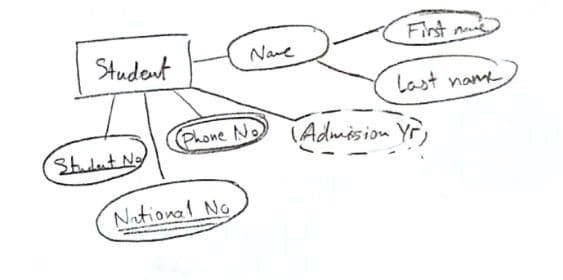
\includegraphics[width = 0.9\textwidth]{Graphics/entity.jpg}
\end{figure}
\section{Relationship}
The interaction between two or more entities is a \textit{relationship}. Mathematically, a relationship is a Cartesian product \(n\) entity types. \(E_1, \dots , E_n\) said to \textit{participate} in a relationship type \(R = E_1 \times \dots \times E_n\) and individual entities \(e_1, \dots , e_n\) are said to \textit{paraticipate} in a relationshiple instance \(r = \bracket{e_1, \dots ,e_n}\). The degree of a relationship is the number of entity types that participate in it. Binary relationship are relationship with two entity types. Binary relationship can have different \textit{cardinality ratios}
\begin{figure}[H]
    \centering
    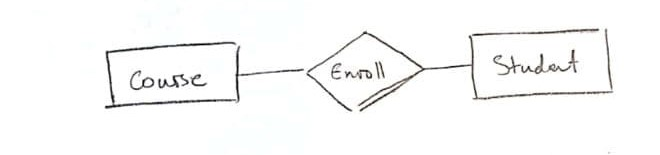
\includegraphics[width = 0.9\textwidth]{Graphics/relationship.jpg}
\end{figure}
\begin{description}
    \item [Many-to-Many] denoted as \(M:N\). For example each STUDENT can enroll in multiple COURSEs and each COURSE has many STUDENT enrolled in it.
    \item [One-to-Many] denoted as \(N:1\). Each DEPARTMENT has many FACULTY but each FACULTY has only one DEPARTMENT. 
    \item [One-to-One] denoted as \(1:1\). Each DEPARTMENT has one DEAN and each DEAN belongs to one DEPARTMENT.
\end{description}[H]
\begin{figure}
    \centering
    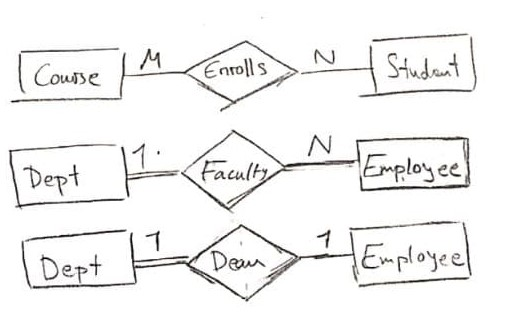
\includegraphics[width = 0.9\textwidth]{Graphics/cardinality.jpg}
\end{figure}
\textit{Total participation} or \textit{existence dependecy} is when each entity in the first entity type must be in a relationship with another entity in the second entity type. For example, each FACULTY must have a DEPARTMENT. In \textit{partial participation} some of the entities in the first entity type are in a relationship with the entities in the second entity type. For example, not every FACULTY is a DEAN. 

A relationship might have attributes for itself. For instance, a DEAN \textit{MANAGES} a DEPARTMENT from a starting time to some other time. 

\section{Weak entity}
An entity type that does not have a key attribute is called a \textit{weak entity}. Those entities that have a key attribute are called \textit{strong entity}. In real world, a weak entity is an entity that is depedent on the existence of another entity, called \textit{identifying/owner entity type}. In ER model we can model this relationship by a total participation relationship which is called \textit{identifying relationship}. A weak entity type normal has one or more \textit{partial key} attributes that distinguish it from the other related weak entities to the same owner entity. For example, a COURSEGROUP entity has the "Semester", "Year", and the "Group Number" attributes of a COURSE entity. Every COURSEGROUP entity must be related to a COURSE entity and here, each of its attributes are partial keys.

By adding weak entities we can reduce the order of a relationship to two and even remove attributes of the relationship and give it to the weak entity.
\begin{figure}
    \centering
    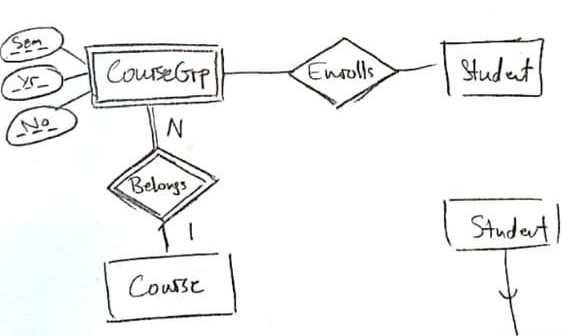
\includegraphics[width = 0.9\textwidth]{Graphics/weak entity.jpg}
\end{figure}
\section{ER notation and diagrams}
Insert the corresponding diagrams :)

\section{Enhanced/Extended ER model}
\subsection{Inheritance}
For inheritance we need a \textit{supertpye} and \textit{subtype} which inherits attributes of the supertype.
We show the concept of inheritance in EER model through \textit{specialization} and \textit{generalization}. Specialization is the process of defining a set of subclasses of an entity type. Generalization is the process of finding common attributes and creating a supertype. A specialization has the following characteristics 
\begin{description}
    \item [Total] every entity of the supertype must be an instance of at least one one the subtypes.
    \item [Partial] opposite of total.
    \item [Disjoint] every entity of the supertype belongs to at most one of the subtypes.
    \item [Overlapping] opposite of disjoint.
\end{description}
Totalness and disjointness are indepedent of each other and hence we can have four combinations. 

\begin{figure}[H]
    \centering
    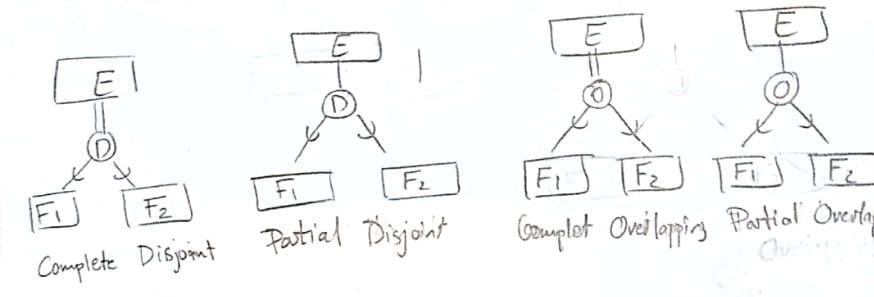
\includegraphics[width = 0.9\textwidth]{Graphics/inheritance.jpg}
\end{figure}
Multiple inheritance can occure when a subtype inherites attributes of one or more supertypes. For example, a TEACHING-ASSISTANT is both a STUDENT and an EMPLOYEE.

\subsection{Union-Type (Category)}
When we want to combine different entities, we use Union types. For example, a VEHICLE can be a CAR or a  TRUCK. 
\begin{description}
    \item [Total] every entity of the subtype is one the supertype.
    \item [Partial] opposite of total.
\end{description}
\begin{figure}[H]
    \centering
    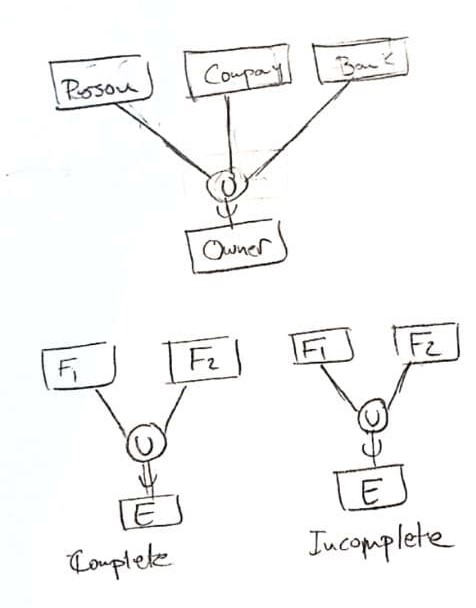
\includegraphics[width = 0.5\textwidth]{Graphics/union.jpg}
\end{figure}

If the keys of the supertpyes are from the same domain, then we can have the same key for the subtype. But, it is better to have different key. Also note that, total union type is equivalent to disjoint total inheritance. 

We represent both inheritance and union-type with a IS-A relationship. 

\section{Aggregation and association}
We need to represent membershipe/being a component/containment relationships as well. IS-A-PART-OF relationships denote the following meanings 
-- insert diagram
\begin{itemize}
    \item F is a part of E.
    \item E contains F.
    \item E has F.
    \item F is a member of E.
\end{itemize}
\begin{figure}
    \centering
    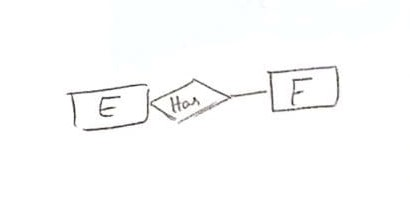
\includegraphics[width = 0.4\textwidth]{Graphics/has}
\end{figure}
We can also view relationships as an entity (i literally have no fucking clue why they dont make a science out of it and standardize it with better capabilities).
\begin{figure}
    \centering
    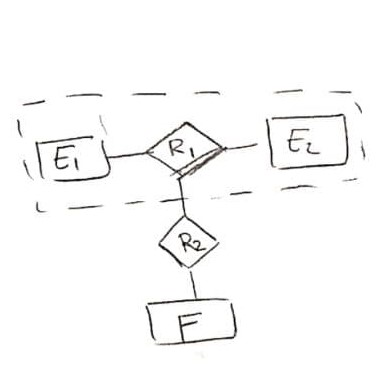
\includegraphics[width = 0.9\textwidth]{Graphics/aggregation.jpg}
\end{figure}
\section{Traps}
There are two traps 
\begin{definition}
    \item [Loop trap] thinking that \((i,s), (s,p) , (p,i) \implies (i,s,p)\) is wrong.
    \item [Chasm trap] failing to model correctly that in a chain of 1:N relationship, the last entity is "connected" to the first entity, because the participation is not total. (If it is ambiguous, let me tell that i have seen a million examples and still dont fucking understand, it is so fucking dumb \_ or maybe i am :\textbackslash).
\end{definition}
\begin{figure}
    \centering
    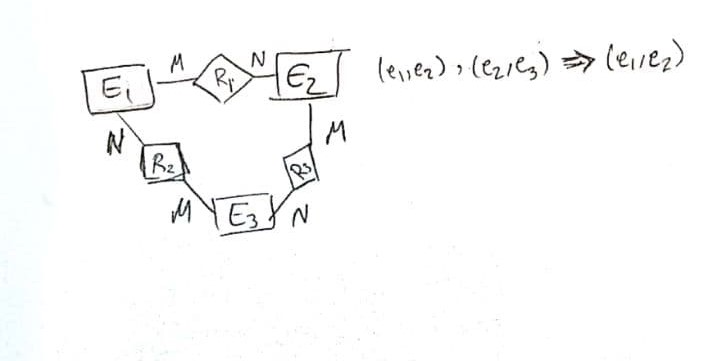
\includegraphics[width = 0.9\textwidth]{Graphics/looptrap.jpg}
\end{figure}